\documentclass[a4paper,onecolumn]{article}
\usepackage{amsmath, amsthm, graphicx, amssymb, wrapfig, fullpage, subfigure, array}
\usepackage[font=sl, labelfont={sf}, margin=1cm]{caption}
\DeclareMathOperator{\e}{e}
\begin{document}
\setcounter{page}{1}
\noindent Coordinate matrix
$$
A = \begin{pmatrix}
    1 & 1 & 1 & 1\\
    x_1 & x_2 & x_3 & x_4\\
    y_1 & y_2 & y_3 & y_4\\
    z_1 & z_2 & z_3 & z_4
\end{pmatrix}
$$
Tetrahedron volume
$$
    V = \frac{1}{6} \textrm{abs}( |A| )
$$
Affine transformation matrix
$$
    F = \frac{1}{\left|A\right|} A
$$
Notice $|A|$ here doesn't have $abs()$, it is the determinant of $A$.
s.t.
$$
    X = \left|A \right| F Z
$$
where
$$
    X = \begin{pmatrix}1\\x\\ y\\z\end{pmatrix}\qquad,\qquad
    Z = \begin{pmatrix}\zeta_1\\\zeta_2\\\zeta_3\\\zeta_4\end{pmatrix}
$$
%$$
%    F^{-1} = 
%    \begin{pmatrix}
%        a_1 & b_1 & c_1 & d_1\\
%        a_2 & b_2 & c_2 & d_2\\
%        a_3 & b_3 & c_3 & d_3\\
%        a_4 & b_4 & c_4 & d_4\\
%    \end{pmatrix}
%$$
Unit tangent vector
$$
    \hat{t}_{ij}=\frac{1}{l_{ij}}\begin{pmatrix}
        (x_j-x_i) \hat{x}\\
        (y_j-y_i) \hat{y}\\
        (z_j-z_i) \hat{z}
    \end{pmatrix}
$$
where $l_{ij}$ is the length of the edge.\\
Define
\begin{equation*}\begin{split}
    \left(i, i_1 , i_2, i_3\right) = &(1\,2\,3\,4)\\&(2\,3\,4\,1)\\&(3\,4\,1\,2)\\&(4\,1\,2\,3)
\end{split}\end{equation*}
Unit normal vector:\\
Step I:
$$
    \hat{n}_i = \frac{ t_{i_1i_2}\times t_{i_1i_3} } {\left|t_{i_1i_2}\times t_{i_1i_3}\right|}
$$
Step II:
$$
    \hat{n}_i = \textrm{sign}\left(\hat{n}_i\cdot \hat{t}_{i i_1}\right)\hat{n}_i
$$
Tetrahedron integration
$$
    \int_V\; \zeta_1^a \zeta_2^b \zeta_3^c \zeta_4^d \; \textrm{d}V = \frac{a!\,b!\,c!\,d!}{(a+b+c+d+3)!} 6V
$$
Twice the opposite triangle area
$$
    S_i = \bigl| l_{i_1i_2} \hat{t}_{i_1 i_2} \times l_{i_1 i_3} \hat{t}_{i_1i_3} \bigr|
$$
Area matrix
$$
    S = \begin{pmatrix}S_1 &&&\\&S_2&&\\&&S_3&\\&&&S_4\end{pmatrix}
$$
Unit vectors
$$
    \hat{\hat{X}} = \begin{pmatrix}
        \hat{0}\\\hat{x}\\\hat{y}\\\hat{z}
    \end{pmatrix}\qquad\qquad
    \hat{\hat{N}} = \begin{pmatrix}
        \hat{n}_1\\\hat{n}_2\\\hat{n}_3\\\hat{n}_4
    \end{pmatrix}
$$
Normal vector outward pointing correction:\\
Type I tetrahedron
$$
  \gamma = 1
$$
Type II tetrahedron
$$
  \gamma = -1
$$
Criterion
\begin{equation*}\begin{split}
    det(A) >0 \qquad \leftrightarrow \qquad &\left( t_{12}\times t_{13} \right) \cdot t_{14} >0\qquad\rightarrow \qquad \textrm{type I}\\
    det(A) <0 \qquad \leftrightarrow \qquad &\left( t_{12}\times t_{13} \right) \cdot t_{14} <0\qquad\rightarrow \qquad \textrm{type II}
\end{split}\end{equation*}
\begin{center}
    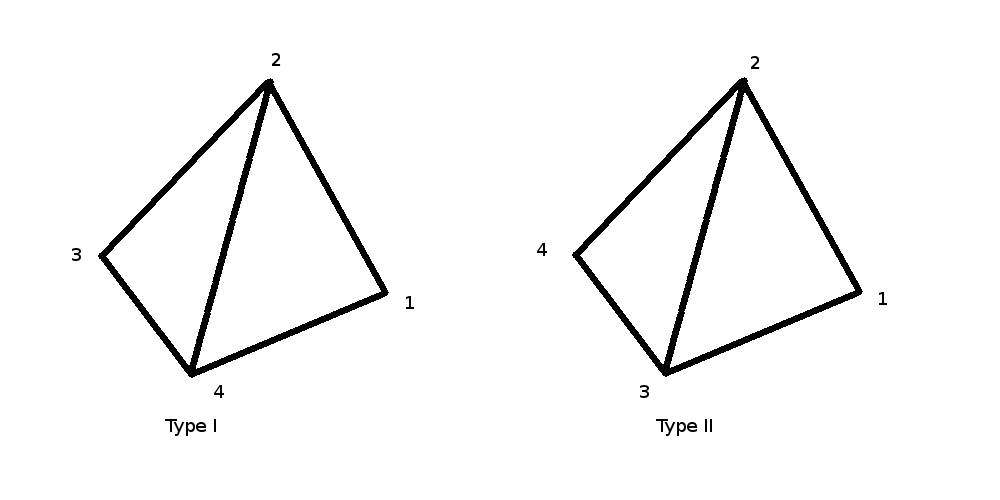
\includegraphics[height=7cm]{typestetra.png}
\end{center}
Conversion
\begin{equation*}\begin{split}
    \hat{\hat{N}} &= -\gamma S^{-1}F^{-1}\hat{\hat{X}}\\
    \hat{\hat{X}} & = -\gamma FS\hat{\hat{N}}
\end{split}\end{equation*}
Nabla
$$
    \nabla \zeta_i = - \frac{S_i}{6 V} \hat{n}_i
$$
$$
    \nabla\times\nabla \zeta_i = 0
$$
where $S_i$ is twice the triangle area.
\begin{figure}\begin{center}
    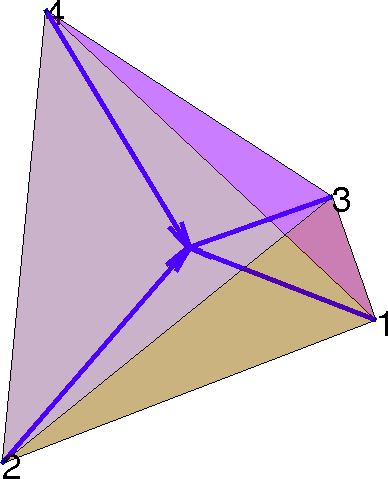
\includegraphics[height=4cm]{normalvectors.png}
    \caption{Outward pointing normal vectors}
\end{center}\end{figure}


\noindent Zeroth-order basis vector
$$
    \hat{N}_{ij} = l_{ij} \left( \zeta_{i}\nabla \zeta_{j} - \zeta_{j} \nabla \zeta_{i} \right)
$$
which satisfies
$$
    \hat{t}_{ij}\cdot \hat{N}_{ij} = 1
$$
Alert $\hat{N}_{ij}$ does not normalize with itself !

\begin{figure}\begin{center}
    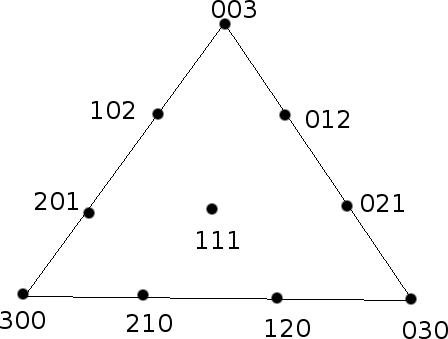
\includegraphics[height=4cm]{code.png}
    \caption{Split code: n=3, split into three segments; m=3, three bits (2D). Put n numbers into m bits. Suitable for both
    global tetrahedron index and sub tetrahedron index.}
\end{center}\end{figure}
\begin{figure}\begin{center}
    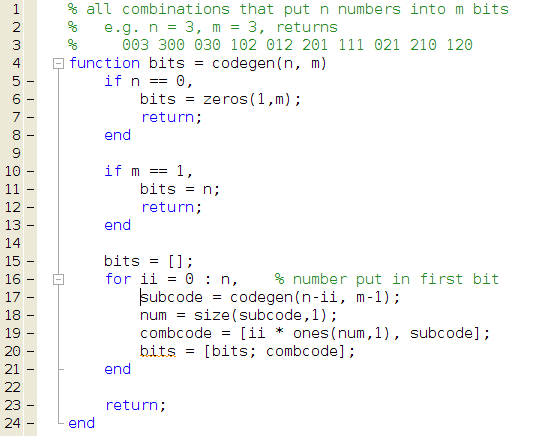
\includegraphics[height=8cm]{codegen.png}
    \caption{Recursive split code generation, Matlab}
\end{center}\end{figure}
\noindent Define order of accuracy $p$, and global split segments (refer to split code) $n$, then
$$
    n = p+2
$$
Relation between global tetrahedron split segments and sub tetrahedron split segments
$$
    n^\prime = n-2
$$
and
$$
    n^\prime = p
$$
\begin{figure}\begin{center}
    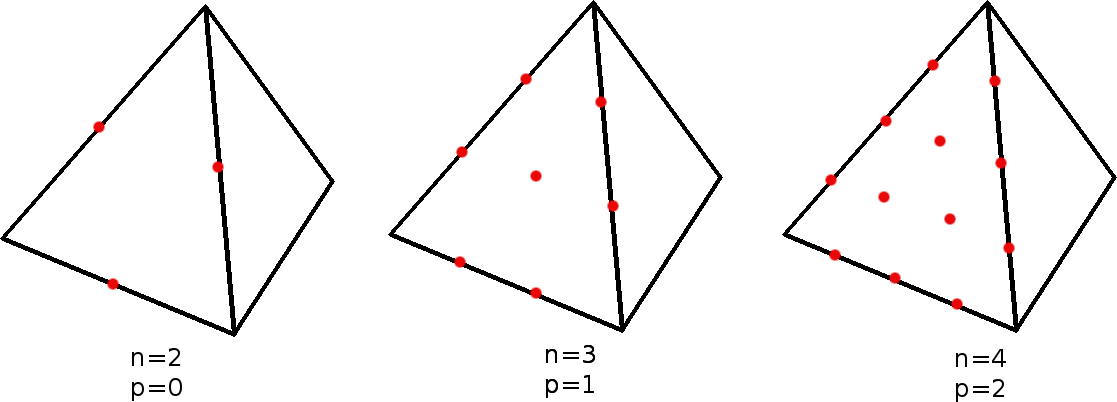
\includegraphics[height=5cm]{interppoint.png}
    \caption{Interpolatory points in a global tetrahedron. Notice \emph{NOT} all points are used
    for generating Lagrangian polynomials for a given edge. Only points associated with a sub tetrahedron
    are used for interpolation. }
\end{center}\end{figure}
Natural coordinates
$$
    Z = \frac{1}{n} \bigl(\textrm{split\_code}\bigr)
$$
\begin{figure}\begin{center}
    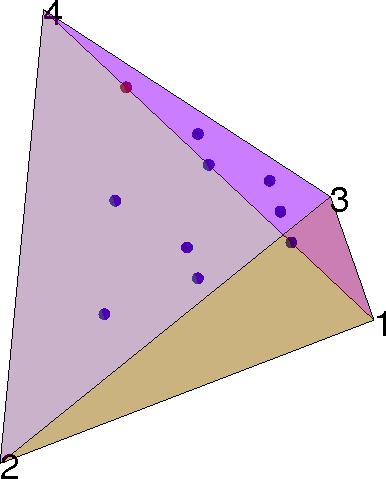
\includegraphics[height=5cm]{interppnt3D.png}
    \caption{Interpolatory points in global tetrahedron along edge 14, n=4 (p=2), m=4 (3D)}
\end{center}\end{figure}
\begin{figure}\begin{center}
    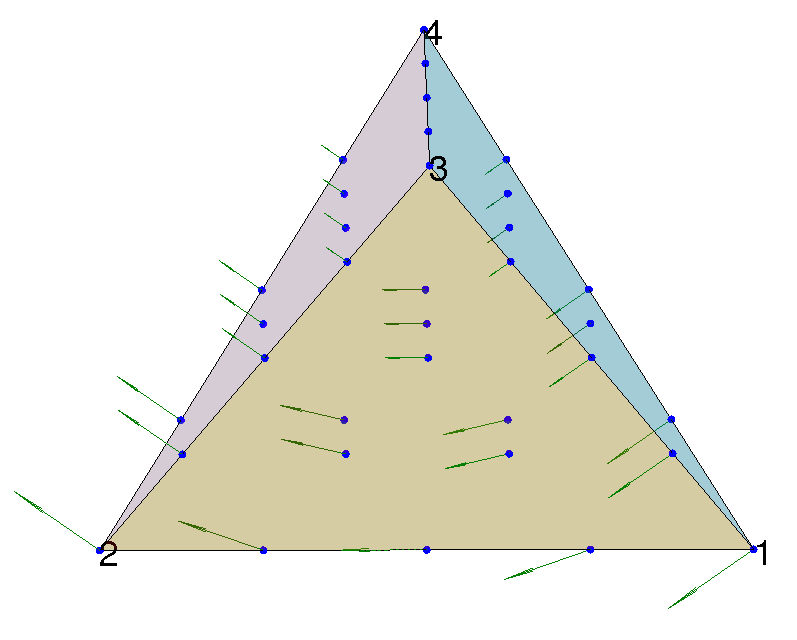
\includegraphics[height=5cm]{quiverbasis.png}
    \caption{$\hat{N}_{12}$}
\end{center}\end{figure}
Differential operators in x-y-z coordinates
$$
    \nabla = \begin{pmatrix}\partial_x \\ \partial_y \\\partial_z\end{pmatrix}
$$
$$
    \nabla\cdot = \begin{pmatrix}\partial_x& \partial_y &\partial_z\end{pmatrix}
$$
$$
    \nabla\times = \begin{pmatrix}
        0 & -\partial_z & \partial_y\\
        \partial_z & 0 & -\partial_x\\
        -\partial_y & \partial_x & 0
    \end{pmatrix}
$$
\begin{equation*}\begin{split}
    \nabla\cdot \hat{N}_{ij} &= 0\\
    \nabla\times \hat{N}_{ij}&=2 l_{ij}\nabla\zeta_i\times \nabla\zeta_j
\end{split}\end{equation*}
For a global tetrahedron, define the split code of an interpolation point to be
$$
    (i,\,j,\,k,\,l)
$$
where
$$
    i+j+k+l=n
$$
For the sub tetrahedron, define split code to be
$$
    (i^\prime,\,j^\prime,\,k^\prime,\,l^\prime)
$$
where
$$
    i^\prime + j^\prime + k^\prime + l^\prime = n^\prime
$$
The interpolation polynomial for point $(i^\prime,j^\prime,k^\prime,l^\prime)$ is
$$
    \Phi_{i^\prime j^\prime k^\prime l^\prime}^{n^\prime} \equiv P_{i^\prime}^{n^\prime}(\zeta_1^\prime)
    P_{j^\prime}^{n^\prime}(\zeta_2^\prime) P_{k^\prime}^{n^\prime}(\zeta_3^\prime) P_{l^\prime}^{n^\prime}(\zeta_4^\prime)
$$
in which
\begin{equation*}\begin{split}
    P_{i^\prime}^{n^\prime}(\zeta^\prime) &= \frac{1}{i^\prime!}\prod_{s=0}^{i^\prime-1} \bigl( n^\prime \zeta^\prime - s \bigr)\\
    P_0^{n^\prime}(\zeta) &= 1
\end{split}\end{equation*}
$\Phi$ is normalized in the sense that
\begin{equation*}\begin{split}
    \Phi_{i^\prime j^\prime k^\prime l^\prime }^{n^\prime}(\frac{i^\prime}{n^\prime},\frac{j^\prime}{n^\prime},\frac{k^\prime}{n^\prime},\frac{l^\prime}{n^\prime}) &= 1\\
    \Phi_{i^\prime j^\prime k^\prime l^\prime }^{n^\prime}(\textrm{otherwise}) &=0
\end{split}\end{equation*}
\begin{figure}\begin{center}
    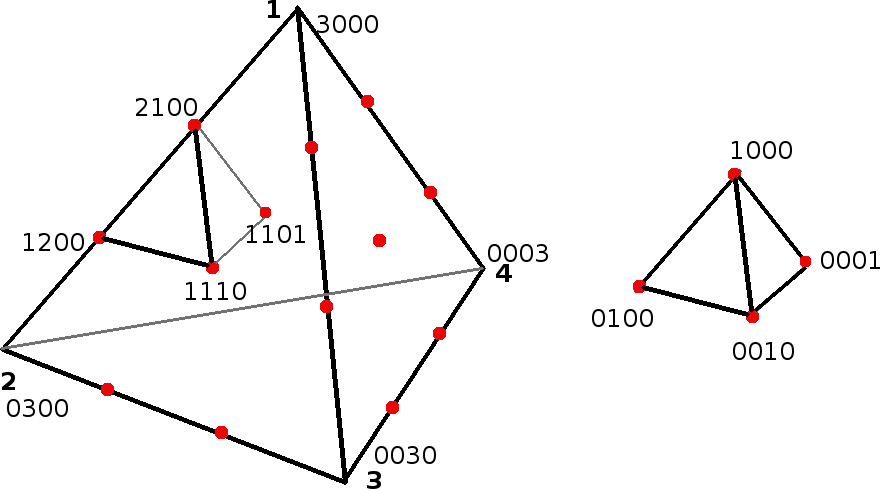
\includegraphics[height=5cm]{subtetraindex.png}
    \caption{$n^\prime=1$, $p=1$, $n=3$. Sub tetrahedron along edge 12. The left (global) tetrahedron uses global split code,
    the right (sub) tetrahedron uses sub split code.}
\end{center}\end{figure}
Although $n^\prime=0$ is not used, we still define its polynomial
$$
    P_0^0=1
$$
$$
    \nabla P_0^0=0
$$
\noindent $n^\prime = 1$ polynomials
\begin{equation*}\begin{split}
    P_0^1(\zeta) &=1\\
    P_1^1(\zeta) &=\zeta
\end{split}\end{equation*}
\begin{equation*}\begin{split}
    \nabla P_0^1 &= 0\\
    \nabla P_1^1 &= 1\nabla \zeta
\end{split}\end{equation*}
\noindent $n^\prime=2$ polynomials
\begin{equation*}\begin{split}
    P_0^2 &=1\\
    P_1^2 &= 2\zeta\\
    P_2^2 &= 2\zeta^2-\zeta
\end{split}\end{equation*}
\begin{equation*}\begin{split}
    \nabla P_0^2 &= 0\\
    \nabla P_1^2 &=2\nabla\zeta\\
    \nabla P_2^2 &= (4\zeta-1)\nabla\zeta
\end{split}\end{equation*}
\noindent $n^\prime=3$ polynomials
\begin{equation*}\begin{split}
    P_0^3(\zeta) &= 1\\
    P_1^3(\zeta) &=3\zeta\\
    P_2^3(\zeta) &=\frac{9}{2}\zeta^2 - \frac{3}{2}\zeta\\
    P_3^3(\zeta) &=\frac{9}{2}\zeta^3-\frac{9}{2}\zeta^2 +\zeta
\end{split}\end{equation*}
\begin{equation*}\begin{split}
    \nabla P_0^3(\zeta) &= 0 \quad=Q_0^3 \nabla\zeta\\
    \nabla P_1^3(\zeta) &=3\nabla\zeta \quad= Q_1^3 \nabla \zeta\\
    \nabla P_2^3(\zeta) &=\left(9\zeta-\frac{3}{2}\right)\nabla \zeta \quad= Q_2^3 \nabla\zeta\\
    \nabla P_3^3(\zeta) &=\left(\frac{27}{2}\zeta^2-9\zeta+1\right)\nabla \zeta\quad=Q_3^3\nabla \zeta
\end{split}\end{equation*}
$n^\prime=4$ polynomials
\begin{equation*}\begin{split}
    P_0^4(\zeta) &= 1\\
    P_1^4(\zeta) &= 4\zeta\\
    P_2^4(\zeta) &= 8 \zeta^2-2\zeta\\
    P_3^4(\zeta) &= \frac{32}{3}\zeta^3 -8\zeta^2+\frac{4}{3}\zeta\\
    P_4^4(\zeta) &=\frac{32}{3}\zeta^4 -16 \zeta^3 + \frac{22}{3}\zeta^2 -\zeta
\end{split}\end{equation*}
\begin{equation*}\begin{split}
    \nabla P_0^4(\zeta) &= 0 \quad= Q_0^4\nabla \zeta\\
    \nabla P_1^4(\zeta) &= 4\nabla \zeta \quad= Q_1^4\nabla\zeta\\
    \nabla P_2^4(\zeta) &= \left(16\zeta-2\right)\nabla \zeta \quad= Q_2^4\nabla\zeta\\
    \nabla P_3^4(\zeta) &= \left(32\zeta^2 - 16\zeta +\frac{4}{3}\right)\nabla \zeta \quad=Q_3^4\nabla\zeta\\
    \nabla P_4^4(\zeta) &= \left(\frac{128}{3}\zeta^3-48\zeta^2 + \frac{44}{3}\zeta-1\right)\nabla \zeta\quad=Q_4^4\nabla\zeta
\end{split}\end{equation*}
$\nabla\Phi_{ijkl}^n$
\begin{equation*}\begin{split}
    \nabla\Phi_{ijkl}^n &= Q_i^nP_j^nP_k^nP_l^n\nabla\zeta_i\\
    &+P_i^nQ_j^nP_k^nP_l^n\nabla\zeta_j\\
    &+P_i^nP_j^nQ_k^nP_l^n\nabla\zeta_k\\
    &+P_i^nP_j^nP_k^nQ_l^n\nabla\zeta_l
\end{split}\end{equation*}
Conversion between global tetrahedron and sub tetrahedron. \\
For example, basis of a sub tetrahedron along \emph{edge 12}
$$
    P^p_{i^\prime}(\zeta_1^\prime) P^p_{j^\prime}(\zeta_2^\prime)P^p_{k^\prime}(\zeta_3^\prime)P^p_{l^\prime}(\zeta_4^\prime) \hat{N}_{12}
$$
Notation: from now on we denote a basis by $b_I$, where $I$ is the global index for the basis.\\
Range
$$
    i^\prime,\, j^\prime,\, k^\prime,\, l^\prime = 0,\,\cdots\,,\,p
$$
Index conversion
\begin{equation*}\begin{split}
    i^\prime &= i-1\\
    j^\prime &= j-1\\
    k^\prime &=k\\
    l^\prime &=l
\end{split}\end{equation*}
Coordinate conversion (change of variables)
\begin{equation*}\begin{split}
    \zeta_1^\prime &= \frac{p+2}{p}\zeta_1-\frac{1}{p}\\
    \zeta_2^\prime &= \frac{p+2}{p}\zeta_2-\frac{1}{p}\\
    \zeta_3^\prime &= \frac{p+2}{p}\zeta_3\\
    \zeta_4^\prime &= \frac{p+2}{p}\zeta_4
\end{split}\end{equation*}
There are
$$
    (p+1)(p+3)(p+4)/2 
$$
basis vectors associated with (but not belong to) an element.
They includes
$$
    6\cdot (p+1)
$$
basis vectors associated with edges;
$$
    4\cdot p(p+1)
$$
basis vectors associated with faces; and
$$
    \frac{1}{2}\cdot (p+1)(p+3)(p+4)
$$
basis vectors associated with interior points.\\
It is verified
\begin{itemize}
    \item An edge associated basis vector is shared by all elements that have that edge.
    \item A face associated basis vector is shared by two elements that have that face.
    \item An interior basis vector is owned by a single element.
\end{itemize}
The first two items ensures the tangential continuity. However, the same basis vector
can represent different normal components in different elements that sharing it.

\section{Finite Element Formulation}
Boundary condition on $S_1$ (electrical conducting, Dirichlet condition)
$$
    \hat{n} \times \vec{E} = 0
$$
Boundary condition on $S_2$ (third kind, natural condition)
$$
    \frac{1}{\mu_r} \hat{n} \times (\nabla \times \vec{E}) + \gamma \hat{n} \times (\hat{n}\times \vec{E}) = \vec{U}
$$
Differential Equation
$$
    \nabla\times \left(\frac{1}{\mu_r}\nabla\times \vec{E}\right)-k_0^2\epsilon_r\vec{E} = -jk_0Z_0\vec{J}
$$
Functional
\begin{equation*}\begin{split}
    F(\vec{E}) &= \frac{1}{2}\int_V \left[ \underbrace{\frac{1}{\mu_r} \left(\nabla\times \vec{E}\right)\cdot \left(\nabla\times\vec{E}\right)}_{1}-
                  \underbrace{k_0^2\epsilon_r \vec{E}\cdot \vec{E}}_{2}\right] \textrm{d}V\\
               &+ \underbrace{\int_{S_2} \left[ \frac{\gamma}{2} \left(\hat{n}\times \vec{E}\right)\cdot \left(\hat{n}\times \vec{E}\right)+\vec{E}\cdot \vec{U} \right] \textrm{d}S}_{4}\\
               &+ j k_0 Z_0 \underbrace{\int_V \vec{E}\cdot \vec{J}\textrm{d}V}_{3}
\end{split}\end{equation*}
Notices:
\begin{itemize}
    \item Code should be carried out for complex number operations.
    \item $\mu_r$, $\epsilon_r$, $\gamma$, $\vec{J}$ are element-wise constant.
\end{itemize}
Enforce Dirichlet boundary condition: for the basis associating $S_1$ surfaces' edges, simply set it to zero. (not verified yet)\\
Elemental matrix from functional part 1:
$$
    \frac{1}{\mu_r^e} \int_{V^e} \left(\nabla\times \vec{b}_I\right)\cdot \left(\nabla\times \vec{b}_J\right) \,\textrm{d}V
$$
Elemental matrix from functional part 2:
$$
    k_0^2 \epsilon_r^e \int_{V^e} \vec{b}_I\cdot\vec{b}_J \,\textrm{d}V
$$
Elemental vector from functional part 3:
$$
    \vec{J}^e \cdot \int_{V^e} \vec{b}_I \,\textrm{d}V
$$
Not consider part 4 yet.
\end{document}






